% !TeX root = ../../thesis.tex
\chapter{Extending the model: adding fluid flow and convection}\label{ch:fluid}

\begin{shaded}
This chapter is partially based on a manuscript prepared to be submitted:\\
M. Barzegari, C. Wang, S.V. Lamaka, G. Zavodszky, and L. Geris, ``Interface-coupled multiphysics computational modeling of local pH changes during the biodegradation of magnesium biomaterials.''
\end{shaded}

Similar to the importance of perfusion in tissue engineering bioreactors, fluid flow plays an important role in biodegradation tests in hydrodynamics conditions. In this chapter, the development of a parallel fluid flow model is detailed, which is further coupled with the biodegradation model for simulating immersion tests in hydrodynamics setup.

\section{Introduction}

Considering fluid flow in the developed biodegradation model is crucial in light of the final application of the model, which is to be coupled with cell differentiation and tissue growth models to predict the rate of neotissue formation on biodegradable implants and scaffolds. In tissue engineering, cell expansion and differentiation experiments usually take place inside perfusion bioreactors, meaning that the flow of a biological fluid provides sufficient nutrients needed for the growth process and removes unnecessary and undesirable waste \cite{Sikavitsas2005,Grayson2010,Sonnaert2014}. Moreover, the induced shear stress resulting from this perfusion plays a prominent role in the cell differentiation process \cite{Song2013,McCoy2012,Rauh2011,Papantoniou2013}, making the fluid flow inside the bioreactor even more critical. Consequently, the effect of the fluid flow should be considered in the biodegradation model to enable it to make predictions in a perfusion setup, which is interchangeably called hydrodynamics conditions in chemistry.

Fluid flow in the context of a hydrodynamic condition has a similar application in corrosion and biodegradation experiments \cite{Wang2014}. In a typical setup, the electrolyte moves and is refreshed over time to remove the corrosion products and provide needed mechanical stimuli if applicable. In biodegradation experiments, the flow velocity and induced shear stress affect the corrosion behavior of degradable scaffolds and implants due to increased mechanical forces and mass transfer \cite{Wang2014}. Studies show that hydrodynamics conditions play a significant role in Mg degradation \cite{Levesque2008} where the corrosion rate increases in comparison to static conditions in immersion tests, in the presence of flowing \cite{Li2012}, rotating \cite{Jafarzadeh2009}, circulating \cite{Chen2010}, and \textit{in vivo} perfusion \cite{Witte2013}. Additionally, the fluid flow helps remove the corrosion products and avoid their accumulation \cite{Hiromoto2008}.

\newglossaryentry{CT}{name={CT},description={computed tomography}}

The effect of hydrodynamics condition on the rate and pattern of biodegradation is rooted in the distribution and diffusion of fluids \cite{Efird2011}, which can be related to increment of mechanical stimuli like wall shear stress or increment in ions transport. It is reported that the presence of fluid flow leading to accelerated movement of the corrosive medium increases the rate of uniform and localized corrosion of Mg alloys \cite{Wang2014}. The increase in corrosion rate is due to the increase of mass transfer of ions \cite{Efird2011}, affecting the chemical reactions occurring in the interface of Mg and the electrolyte \cite{Hiromoto2008,Xu2009}. Moreover, the increment in mass transfer removes more corrosion products from the surface, which is another contribution of the fluid flow to increasing the biodegradation rate \cite{Efird2011}. Wang et al. \cite{Wang2014} reported that the degradation rate was $0.37\pm0.007$ and $1.21\pm0.27 \text{mm.year}^{-1}$ for the corrosion of stents made of Mg AZ31 alloys in static and hydrodynamics conditions, respectively. After considering the volume loss with \gls{CT} measurements, they have concluded that the corrosion rate of these alloys is three times more in the presence of fluid flow, increasing from $\sim 0.6\text{mm.year}^{-1}$ in static condition to $\sim 1.5\text{mm.year}^{-1}$ in a hydrodynamics setup \cite{Wang2014}. This shows the significance of adding fluid flow to the developed biodegradation model.

Computational Fluid Dynamics (\gls{CFD}) is the field of studying the dynamics of fluid flow using mathematical and computational methods \cite{H.Versteeg2007,Sharma2022}. The fluid flow is usually expressed in the form of Navier-Stokes or Stokes equations, on which appropriate numerical schemes are applied and the derived system of equations is solved using computers, resulting in the prediction of flow patterns and secondary entities like the shear stress. \gls{CFD} modeling has been used in tissue engineering to study fluid flow systems such as dynamic cell culture conditions in perfusion bioreactors \cite{Hutmacher2008, Hossain2012,Patrachari2012}.

In this chapter, a parallel computational model for fluid flow simulations was developed and coupled with the biodegradation model. The model was developed by solving the derived equations, i.e., Navier-Stokes equations coupled with the Darcy effect for the degrading object, using the finite element method. To ensure proper verification of the simulation results, the model output was compared with an OpenFOAM simulation on the same geometry and setup.

\section{Methods}

\subsection{Navier-Stokes equations}

In its general form, the Navier-Stokes equations describing the flow of an incompressible fluid with constant density $\rho$ in the domain $\Omega \subset \mathbb{R}^{d}$ (with $d$ being the dimension, so 2 or 3) can be written as \cite{Chung2014}:
\begin{equation} \label{eq:fluid_ns_general}
\left\{ {\begin{array}{*{20}{l}}
\displaystyle  {\frac{{\partial {\mathbf{u}}}}{{\partial t}} - {\nabla\cdot}[\nu(\nabla {\mathbf{u}} + \nabla {{\mathbf{u}}^T})] + ({\mathbf{u}}.\nabla ){\mathbf{u}} + \nabla p = {\mathbf{f}},\quad x \in \Omega ,t > 0,} \\
\displaystyle  {\nabla\cdot{\mathbf{u}} = 0,\quad \quad \quad \quad \quad \quad \quad \quad \quad \quad \quad \quad \quad \quad x \in \Omega ,t > 0,}
\end{array}} \right.
\end{equation}
in which $\mathbf{u}$ is the fluid velocity, $p$ is the pressure (which is actually pressure divided by the density), $\nu = \frac{\mu}{\rho}$ is the kinematic viscosity (with $\mu$ being the dynamic viscosity), and
$\mathbf{f}$ is a force term. The equations are conservation of linear momentum and conservation of mass (also called continuity equation), respectively. When $\nu$ is constant, the diffusion term in Eq. \ref{eq:fluid_ns_general} can be simplified as \cite{Quarteroni2014}:
\begin{equation}
\text{div} [\nu(\nabla {\bf u}+\nabla {\bf u}^{T})] =\nu (\Delta {\bf u} + \nabla \text{div} {\bf u})=\nu \Delta {\bf u},
\end{equation}
which turns Eq. \ref{eq:fluid_ns_general} into the following form:
\begin{equation}  \label{eq:fluid_ns}
\left\{ {\begin{array}{*{20}{l}}
\displaystyle  {\frac{{\partial {\mathbf{u}}}}{{\partial t}} - \nu\Delta{\mathbf{u}} + \left( {{\mathbf{u}} \cdot \nabla } \right) {\mathbf{u}} + \nabla p = {\mathbf{f}},\quad x \in \Omega ,t > 0,} \\
 \displaystyle {\nabla\cdot{\mathbf{u}} = 0,\quad \quad \quad \quad \quad \quad \quad \quad \quad \quad \quad \quad \quad \quad x \in \Omega ,t > 0,}
\end{array}} \right.
\end{equation}

Eq. \ref{eq:fluid_ns} satisfies the incompressibility condition $\nabla\cdot\mathbf{u}=0$ and needs proper initial and boundary conditions to be well-posed. The initial condition can be defined as:
\begin{equation}
{\bf u}({\bf x},0)={\bf u}_{0}({\bf x})\qquad \forall{\bf x}\ \epsilon\ {\bf \Omega,}
\end{equation}
where ${\bf u}_{0}$ is a divergence-free velocity field. Various types of boundary conditions can be applied, but the ones we deal with in this chapter are described here. If $\partial \Omega$ is the boundary of $\Omega$, it can be split into 3 distinct boundaries $\partial \Omega=\Gamma_{1} \cup \Gamma_{2} \cup \Gamma_{3}$ each of which with a different type. On $\Gamma_{1}$, the inlet can be defined as a Dirichlet boundary condition for the velocity for a given velocity profile ${\bf g}$:
\begin{equation}
{\bf u} = {\bf g} \quad \text{on } \Gamma_1
\end{equation}

On $\Gamma_2$, a wall boundary no-slip condition can be considered:
\begin{equation}
{\bf u} = 0 \quad \text{on } \Gamma_2
\end{equation}

On $\Gamma_3$, for the outlet condition, a homogeneous Neumann condition on velocity and a zero pressure condition can be defined like:
\begin{equation} \label{eq:fluid_gamma3}
\frac{\partial {\bf u}}{\partial \boldsymbol{n}} = 0, \quad p = 0, \quad \text{on } \Gamma_3
\end{equation}
with $\boldsymbol{n}$ being the normal direction on the boundary $\partial \Omega$. Broadly speaking, these boundaries can be grouped into 2 sets: $\Gamma_{D} = \Gamma_{1} \cup \Gamma_{2}$ and $\Gamma_{N} = \Gamma_{3}$ for boundaries with Dirichlet and Neumann conditions, respectively.

The Navier-Stokes equations can be written componentwise for individual components of the flow vector field in the Cartesian coordinates. Denoting $u_i, i=1,\ldots,d$ (with $d=2$ in 2D and $d=3$ in 3D), Eq. \ref{eq:fluid_ns} can be presented as:

\begin{equation}
\left\{ {\begin{array}{*{20}{l}}
\displaystyle  {\frac{{\partial {u_i}}}{{\partial t}} - \nu \Delta {u_i} + \mathop \sum \limits_{j = 1}^d {u_j}\frac{{\partial {u_i}}}{{\partial {x_j}}} + \frac{{\partial p}}{{\partial {x_i}}} = {f_i},\qquad i = 1, \ldots ,d,} \\
\displaystyle  {\mathop \sum \limits_{j = 1}^d \frac{{\partial {u_j}}}{{\partial {x_j}}} = 0.}
\end{array}} \right.
\end{equation}


\subsection{Weak formulation of the Navier-Stokes equations} \label{sec:fluid_weak}

For deriving the weak formulation, the first equation of \ref{eq:fluid_ns} is multiplied by a test function $\bf v$ defined on a proper function space V (with ${\bf H}^{1}$ being the Sobolev space defined in domain $\Omega$) in which the test functions vanish on the Dirichlet boundary:
\begin{equation} \label{eq:fluid_space_v}
V = [{\bf H}^{1}_{\Gamma_{D}}(\Omega)]^{d} = \lbrace{\bf V} \in [{\bf H}^{1}(\Omega)]^{d} : {\bf v}|_{\Gamma_{D}} = {\bf 0}\rbrace.
\end{equation}
yielding to:
\begin{equation} \label{eq:fluid_weak1}
{\mathop{\int}_{\Omega}} {\partial {\bf u} \over \partial t}.{\bf v}\ d\omega- {\mathop{\int}_{\Omega}}\nu\triangle{\bf u.v}d\omega+ {\mathop{\int}_{\Omega}}[({\bf u.\nabla){\bf u].{\bf v}}}d\omega+ {\mathop{\int}_{\Omega}}\nabla p.{\bf v}d\omega= {\mathop{\int}_{\Omega}}{\bf f. v}d\omega.
\end{equation}

\noindent Applying Green's divergence theory results in:
\begin{equation} \label{eq:fluid_green1}
-\int_{\Omega} \nu \Delta \mathbf{u} \cdot \mathbf{v} d \omega=\int_{\Omega} \nu \nabla \mathbf{u} \cdot \nabla \mathbf{v} d \omega-\int_{\partial \Omega} \nu \frac{\partial \mathbf{u}}{\partial \mathbf{n}} \cdot \mathbf{v} d \gamma
\end{equation}
and
\begin{equation} \label{eq:fluid_green2}
\int_{\Omega} \nabla p \cdot \mathbf{v} d \omega=-\int_{\Omega} p \nabla\cdot \mathbf{v} d \omega+\int_{\partial \Omega} p \mathbf{v} \cdot \mathbf{n} d \gamma
\end{equation}

\noindent Substituting Eqs. \ref{eq:fluid_green1} and \ref{eq:fluid_green2} into Eq, \ref{eq:fluid_weak1} yields to:
\begin{equation} \label{eq:fluid_ns_weak}
\begin{array}{r}
\displaystyle\int_{\Omega} \frac{\partial \mathbf{u}}{\partial t} \cdot \mathbf{v} d \omega+\int_{\Omega} \nu \nabla \mathbf{u} \cdot \nabla \mathbf{v} d \omega+\int_{\Omega}[(\mathbf{u} \cdot \nabla) \mathbf{u}] \cdot \mathbf{v} d \omega-\int_{\Omega} p \nabla\cdot \mathbf{v} d \omega \\
\displaystyle=\int_{\Omega} \mathbf{f} \cdot \mathbf{v} d \omega+\int_{\partial \Omega}\left(\nu \frac{\partial \mathbf{u}}{\partial \mathbf{n}}-p \mathbf{n}\right) \cdot \mathbf{v} d \gamma \quad \forall \mathbf{v} \in V .
\end{array}
\end{equation}

\noindent The last term of Eq. \ref{eq:fluid_ns_weak} is expressed in accordance to the defined Neumann boundary condition, which vanishes on $\Gamma_3$ due to the defined condition in the current study (Eq. \ref{eq:fluid_gamma3}). Moreover, this term vanishes on the Dirichlet boundaries due to the properties of the function space $V$ (Eq. \ref{eq:fluid_space_v}).

Similarly, the second equation of \ref{eq:fluid_ns} is multiplied by a test function $q$ belonging to the function space Q (with ${\bf L}^2$ being a Hilbert space defined in domain $\Omega$), called the pressure space:
\begin{equation}
Q = {\bf L}^2_0(\Omega) = \lbrace p \in {\bf L}^2(\Omega) : {\mathop{\int}_{\Omega}} p \ d\omega = 0\rbrace,
\end{equation}
resulting in:
\begin{equation} \label{eq:fluid_ns_weak_pressure}
{\mathop{\int}_{\Omega}} q \nabla\cdot{\bf u}\ d\omega = 0 \qquad \forall q \in Q.
\end{equation}

Eqs. \ref{eq:fluid_ns_weak} and \ref{eq:fluid_ns_weak_pressure} are so called weak forms of the Navier-Stokes equations.

\subsection{Stokes equations}

For viscous flow, where the Reynolds number is less than 1 ($Re = {|{\bf U}|L \over \nu}$, with $L$ and $\bf U$ being the representative length and velocity of the domain), the convection term of the Navier-Stokes equations can be neglected, simplifying Eq. \ref{eq:fluid_ns} to \cite{Quarteroni2014}:
\begin{equation} \label{eq:fluid_stokes}
\left\{ {\begin{array}{*{20}{l}}
\displaystyle  {\alpha \mathbf{u} - \nu\Delta \mathbf{u} + \nabla p = \mathbf{f} \quad \text{in}\;\Omega ,} \\
\displaystyle  {\nabla\cdot\mathbf{u} = 0\quad \quad \quad \quad \;\;\;\text{in}\;\Omega ,}
\end{array}} \right.
\end{equation}
with $\alpha$ being a positive coefficient. Eq. \ref{eq:fluid_stokes} can be used to model laminar flow in low Reynolds regimes and is simpler to handle than Eq. \ref{eq:fluid_ns} from the numerical computing perspective. The weak formulation of the Stokes equation can be derived by following the approach taken for the Navier-Stokes equations in Section \ref{sec:fluid_weak}. The final form of the weak formulation is:
\begin{equation} \label{eq:fluid_stokes_weak}
\left\{ {\begin{array}{*{20}{l}}
\displaystyle  {\int\limits_\Omega  {(\alpha {\mathbf{u}}.{\mathbf{v}} + \nu\nabla {\mathbf{u}}.\nabla {\mathbf{v}})\,} d\omega  - \int\limits_\Omega  {p\nabla\cdot{\mathbf{v}}\;d\omega  = } \int\limits_\Omega  {{\mathbf{f}}.{\mathbf{v}}\;d\omega \qquad {\forall {\mathbf{v}}} \in V,} } \\
\displaystyle  {\int\limits_\Omega  {q\nabla\cdot{\mathbf{u}}\;d\omega  = 0} \qquad \qquad \qquad \qquad \qquad \qquad \qquad \;\;\;{\forall {{q}}} \in Q,}
\end{array}} \right.
\end{equation}

Eq. \ref{eq:fluid_stokes_weak} can be written in the standard finite element variational form by defining 2 bilinear terms $a: V \times V \mapsto \mathbb{R}$ and $b: V \times Q \mapsto \mathbb{R}$:
\begin{equation}
\begin{array}{*{20}{l}}
\displaystyle  {a({\mathbf{u}},{\mathbf{v}}) = \int\limits_\Omega  {(\alpha {\mathbf{u}}.{\mathbf{v}} + \nu\nabla {\mathbf{u}}.\nabla {\mathbf{v}})\;d\omega ,} } \\
\displaystyle  {b({\mathbf{u}},{q}) =  - \int\limits_\Omega  {q\nabla\cdot{\mathbf{u}}\;d\omega ,} }
\end{array}
\end{equation}
which simplifies the notation of the variational problem of the Stokes equation to:
\begin{equation}
\left\{ {\begin{array}{*{20}{l}}
\displaystyle  {a({\mathbf{u}},{\mathbf{v}}) + {b}({\mathbf{v}},p) = ({\mathbf{f}},{\mathbf{v}})\qquad {\forall {\mathbf{v}}} \in V,} \\
\displaystyle  {b({\mathbf{u}},q) = 0\qquad \qquad \qquad \quad \;{\forall q} \in Q,}
\end{array}} \right.
\end{equation}
in which
\begin{equation}
(\mathbf{f}, \mathbf{v})=\sum_{i=1}^{d} \int_{\Omega} f_{i} v_{i} d \omega.
\end{equation}


\subsection{Implementation}

Numerical implementation of the Stokes (Eq. \ref{eq:fluid_stokes}) and Navier-Stokes (Eq. \ref{eq:fluid_stokes}) equations can be tricky due to the presence of specific sources of instability, which highly depends on the type of studied fluid regime \cite{Girault1979, Elman2014}. Various numerical models have been presented for dealing with these equations, some of which are commonly used in \gls{CFD} applications, such as the Newton-Raphson approximation of Navier-Stokes equations and the Chorin's projection method.

In order to increase the stability and avoid problems in the mathematical analysis of the numerical models (e.g., V-ellipticity
property), a pseudo-compressibility assumption can be added to the continuity equation. The pseudo-compressible approximation appears as a pressure term $\varepsilon p$ with $\varepsilon$ being a very small coefficient, resulting in the following equation as the final form of the Navier-Stokes equations that we consider in this study \cite{devuyst2013}:
\begin{equation}  \label{eq:fluid_ns_pseudo}
\left\{ {\begin{array}{*{20}{l}}
\displaystyle  {\frac{{\partial {\mathbf{u}}}}{{\partial t}} - \nu\Delta{\mathbf{u}} + \left( {{\mathbf{u}} \cdot \nabla } \right) {\mathbf{u}} + \nabla p = {\mathbf{f}},} \\
 \displaystyle {\nabla\cdot{\mathbf{u}} + \varepsilon p = 0.}
\end{array}} \right.
\end{equation}

Similarly, the Stokes equation can be written as:
\begin{equation} \label{eq:fluid_stokes_pseudo}
\left\{ {\begin{array}{*{20}{l}}
\displaystyle  {\alpha \mathbf{u} - \nu\Delta \mathbf{u} + \nabla p = \mathbf{f},} \\
\displaystyle  {\nabla\cdot\mathbf{u} + \varepsilon p = 0.}
\end{array}} \right.
\end{equation}

\newglossaryentry{ODE}{name={ODE},description={ordinary differential equation}}

Another challenging part is to approximate the convection terms in the equations. One of the best approaches to do so is to take advantage of the method of characteristics, in which the characteristics curves of a \gls{PDE} are used to convert it to an \gls{ODE}, resulting in a simpler solution. By using the method of characteristics for the convection term and a backward Euler discretization for the temporal term, the weak form of the Navier-Stokes and continuity equations (Eq. \ref{eq:fluid_ns_pseudo}) can be rewritten as:
\begin{equation} \label{eq:fluid_ns_weak_implement}
\begin{aligned}
&\int_{\Omega} \frac{\mathbf{u}^{n+1}-\mathbf{u}^{n} \circ X^{n}}{\Delta t} \cdot \mathbf{v} d \omega+\nu \int_{\Omega} \nabla \mathbf{u}^{n+1} \cdot \nabla \mathbf{v} d \omega-\int_{\Omega} p^{n+1} \nabla \cdot \mathbf{v} d \omega=\int_{\Omega} \mathbf{f} \cdot \mathbf{v} d\omega \\
&\int_{\Omega} \nabla \cdot \mathbf{u}^{n+1} q d \omega+\varepsilon \int_{\Omega} p^{n+1} q d \omega=0
\end{aligned}
\end{equation}
in which $(\mathbf{u}^{n+1},p^{n+1})$ are the unknowns to be computed from the known state $\mathbf{u}^{n}$ coming from the previous time step or the initial condition. In Eq. \ref{eq:fluid_ns_weak_implement}, the term $\mathbf{u}^{n+1}-\mathbf{u}^{n} \circ X^{n}$ is corresponding to the convection term being approximated using the method of characteristics.

The weak form of the Stokes equations stays almost the same as Eq. \ref{eq:fluid_stokes_weak} (because it does not contain transient and convection terms) but needs a slight modification to add the pseudo-compressible terms from Eq. \ref{eq:fluid_stokes_pseudo}:
\begin{equation} \label{eq:fluid_stokes_weak_implement}
\begin{array}{*{20}{l}}
\displaystyle  {\int\limits_\Omega  {(\alpha {\mathbf{u}}.{\mathbf{v}} + \nu\nabla {\mathbf{u}}.\nabla {\mathbf{v}})\,} d\omega  - \int\limits_\Omega  {p\nabla\cdot{\mathbf{v}}\;d\omega  = } \int\limits_\Omega  {{\mathbf{f}}.{\mathbf{v}}\;d\omega,} } \\
\displaystyle  {\int\limits_\Omega  {q\nabla\cdot{\mathbf{u}}\;d\omega +\varepsilon \int_{\Omega} p q d \omega  = 0}.}
\end{array}
\end{equation}

The model was implemented in the open-source \gls{PDE} solver FreeFEM \cite{Hecht2012} using P1 elements for the pressure and P2 elements for the velocity state variables. Eqs. \ref{eq:fluid_ns_weak_implement} and \ref{eq:fluid_stokes_weak_implement} can be easily implemented in FreeFEM thanks to the built-in support of the method of characteristics via the \verb|convect| function.


\subsection{Preconditioning and parallelizing the computation}

The solution of the Stokes and Navier-Stokes equations using the finite element method in 3D is a computationally intensive process, and as a result, taking advantage of high-performance techniques to reduce the simulation time becomes crucial in real-world applications. Preconditioning the system and parallelizing the simulation by partitioning the mesh and distributing the partitions among available computing nodes in a parallel computing setup are great solutions to this challenge.

In the current implementation, the METIS graph partitioner \cite{METIS1998} and \gls{HPDDM} package \cite{Jolivet2013} were used to partition the computational mesh and distribute the load over the available resources. For preconditioning and improving the solution time of the derived equations, various (combinations of) preconditioners and iterative or direct solvers available in the \gls{PETSc} toolkit \cite{petsc} were tested to find the most suitable combination.

While exact factorization preconditioners (such as LU) are easy to implement and use for fluid flow applications, they show bad memory scaling profiles in large-scale problems, meaning that memory usage increases exponentially with the problem size, making it almost impossible to use them for 3D cases. A better solution for this class of problems is to take advantage of the FieldSplit preconditioner in the \gls{PETSc} toolkit, which allows solving the derived linear system of equations using the block matrices technique. In this technique, the matrices are divided into smaller blocks, and separate preconditioners or solvers can be assigned to each block (each field). These blocks arise naturally from the underlying physics or numerical discretization of the problem, such as velocity and pressure in fluid flow applications. For matrices with an arbitrary number of blocks, three different ``block'' algorithms are available in the \gls{PETSc} toolkit: block Jacobi (\verb|additive|), block Gauss-Seidel (\verb|multiplicative|), and symmetric block Gauss-Seidel (\verb|symmetric_multiplicative|), which can be selected by passing the desired one to the \verb|pc_fieldsplit_type| flag. For two blocks, like the one in fluid flow problems with velocity and pressure as the blocks, another family of solvers based on Schur complements can be used.

\newglossaryentry{AMG}{name={AMG},description={algebraic multigrid}}
\newglossaryentry{KSP}{name={KSP},description={Krylov subspace}}

In the current study, the FieldSplit preconditioner with Schur complement approximation was used on two blocks for velocity and pressure. A \gls{GMRES} \gls{KSP} type \cite{Saad1986} was employed to solve the preconditioned system with an iterative solver. An Algebraic Multigrid (\gls{AMG}) preconditioner \cite{mccormick1987} was used for the velocity block, and a Jacobi preconditioner was assigned to the pressure block. The result of this configuration, as well as the request for appropriate monitoring tools, can be written as follows:
\begin{verbatim}
-ksp_monitor -ksp_converged_reason -ksp_type fgmres
-pc_type fieldsplit -pc_fieldsplit_type schur
-pc_fieldsplit_schur_fact_type full
-fieldsplit_velocity_pc_type gamg
-fieldsplit_velocity_ksp_type preonly
-fieldsplit_pressure_pc_type jacobi
-fieldsplit_pressure_ksp_max_it 5 \end{verbatim}
to pass to \gls{PETSc} while solving the equations.


\subsection{Considering the degrading object}

In biodegradation simulations, a degrading object exists in the fluid domain, through which the flow should not pass because it is a solid part. One common approach to handle this situation is to remove the solid part from the fluid flow mesh, but since the part shrinks over time, this is not a feasible and efficient approach, needing tremendous mesh recreation and removal during simulation. As a result, in the current study, the presence of the solid body as a barrier is taken into account by adding a Darcy term for the permeability to the Navier-Stokes and Stokes equations. A penalization technique is then employed to implement it in the weak formulation. To couple the fluid flow model with the biodegradation model, a convection term is added to the ions transport equations, causing the fluid velocity field advect the ions.

Adding the Darcy  term to Eq. \ref{eq:fluid_stokes} and considering no other acting force yields to:
\begin{equation} \label{eq:fluid_stokes_permeab}
- \nu\Delta \mathbf{u} + \nabla p + \frac{\nu}{K} \mathbf{u} = 0,
\end{equation}
where $K$ is the permeability function.  Similar to Eq. \ref{eq:fluid_stokes_permeab} the effect of the solid part can be added to the Navier-Stokes equation (Eq. \ref{eq:fluid_ns}) by the Darcy term, leading to the following equation:
\begin{equation}  \label{eq:fluid_ns_permeab}
\frac{{\partial {\mathbf{u}}}}{{\partial t}} - \nu\Delta{\mathbf{u}} + \left( {{\mathbf{u}} \cdot \nabla } \right) {\mathbf{u}} + \nabla p + \frac{\nu}{K} \mathbf{u} = 0.
\end{equation}

The Darcy term vanishes in regions with high permeability, i.e., inside the fluid domain, resembling the Stokes equation. Still, when $K$ is very small, i.e., inside the solid part, it dominates the flow and acts like a barrier. To avoid numerical perturbation for switching between these 2 regions, a Heaviside function is defined to update $K$ \cite{Guyot2016}:
\begin{equation}
H(\phi)=\left\{\begin{array}{l}
0, \quad \phi<-\varepsilon \\
\frac{1}{2}+\frac{\phi}{2 \varepsilon}+\frac{1}{2 \pi} \sin \left(\frac{\pi \phi}{\varepsilon}\right), \quad-\varepsilon<\phi<\varepsilon \\
1, \quad \phi>-\varepsilon
\end{array}\right.
\end{equation}
in which $\phi$ is the level-set signed distance function used to separate the solid and solution parts (Eqs. \ref{eq:lsm_full} and \ref{eq:lsm_simplified}), and $\varepsilon$ is set to 1.5h, with h being the minimum mesh element size. Then, $K$ can be accordingly updated to have a smooth transition between regions with a big difference in permeability:
\begin{equation}
K(\boldsymbol{x})=10^{30}(1-H)+K_{0} H
\end{equation}
where $K_{0}$ is the permeability of metals in fluid regions ($\sim10^{-6}$ H/m).

\subsection{Simulation setup}

\subsubsection{Test case to compare with OpenFOAM}

\newglossaryentry{SIMPLE}{name={SIMPLE},description={semi-implicit method for pressure linked equations}}

In order to perform a verification analysis on the developed \gls{CFD} model, a case of 3D flow inside a chamber was implemented to compare the simulation results with those of a well-established and known \gls{CFD} solver. For this reason, the OpenFOAM open-source solver was used, which has been extensively used for fluid dynamics simulations over the last decades \cite{Weller1998}. The simulation was carried out using the simpleFOAM solver, which uses the \gls{SIMPLE} (Semi-Implicit Method for Pressure Linked Equations) algorithm for coupling and solving the Navier-Stokes equations.

\begin{figure}[h]
\centering
\medskip
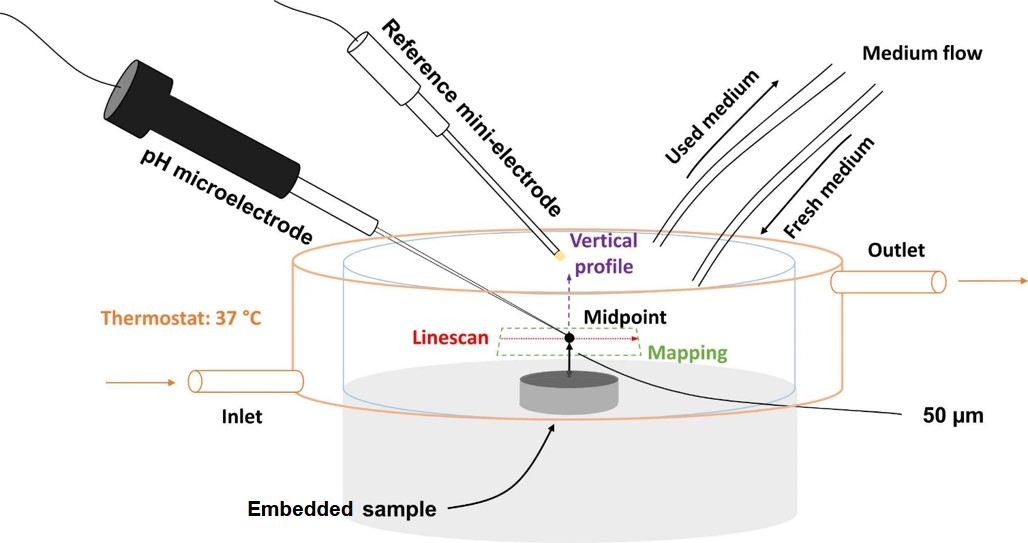
\includegraphics[width=\textwidth]{setup.jpg}
\caption[Fluid flow model construction for comparison with experimental setup]{Fluid flow model construction for comparing the \gls{CFD} results with the experimental setup: a) a schematic of the experimental setup, b) the CAD geometry, c) the generated mesh containing tetrahedral elements.} \label{fig:fluid_setup}
\end{figure}

The geometry was chosen based on the experiments performed for biodegradation in hydrodynamics conditions. The experimental setup is depicted in Fig. \ref{fig:fluid_setup}-A, where the constructed CAD geometry is shown in Fig. \ref{fig:fluid_setup}-B. The computational mesh, comprising linear tetrahedral elements, was generated using Netgen \cite{Schoeberl1997} in the SALOME platform \cite{Ribes2007}. The final mesh used in both FreeFEM and OpenFOAM models is shown in Fig. \ref{fig:fluid_setup}-C, containing \num{100888} elements.

The fluid flow direction is from left to right, meaning that the inlet was set on the vertical face of the small pipe on the bottom left side of the chamber, and the outlet was set similarly on the upper right pipe. The rest of the boundaries were set to no-slip boundary conditions. A zero pressure boundary condition was set on the outlet. The inlet velocity was set to $1.0 \mathrm{mm}/\mathrm{s}$, and the parameter $\nu$ was set to $0.85 \mathrm{mm}^2/\mathrm{s}$.

\subsubsection{Test case to check coupling with degradation model}

In addition to the test case for verification of the developed \gls{CFD} code, two more cases were constructed to evaluate the model's performance in the presence of a barrier, i.e., the degrading object in the coupled biodegradation model. To this end, after coupling the models, a simple 3D geometry of a cylinder with an embedded sphere as the degrading object inside was simulated. The simulation parameters were set similarly to the verification case. The inlet and outlet were assigned to the bases of the cylinder, and the altitude was assigned as the wall boundary condition. Fig. \ref{fig:fluid_coupled_setup} shows a schematic of the computational setup for this test case as well as a vertical cut of the generated computational mesh containing \num{640249} elements. The mesh was refined on the interface of the degrading object to increase the numerical accuracy of the biodegradation model.


\begin{figure}[h]
\centering
\medskip
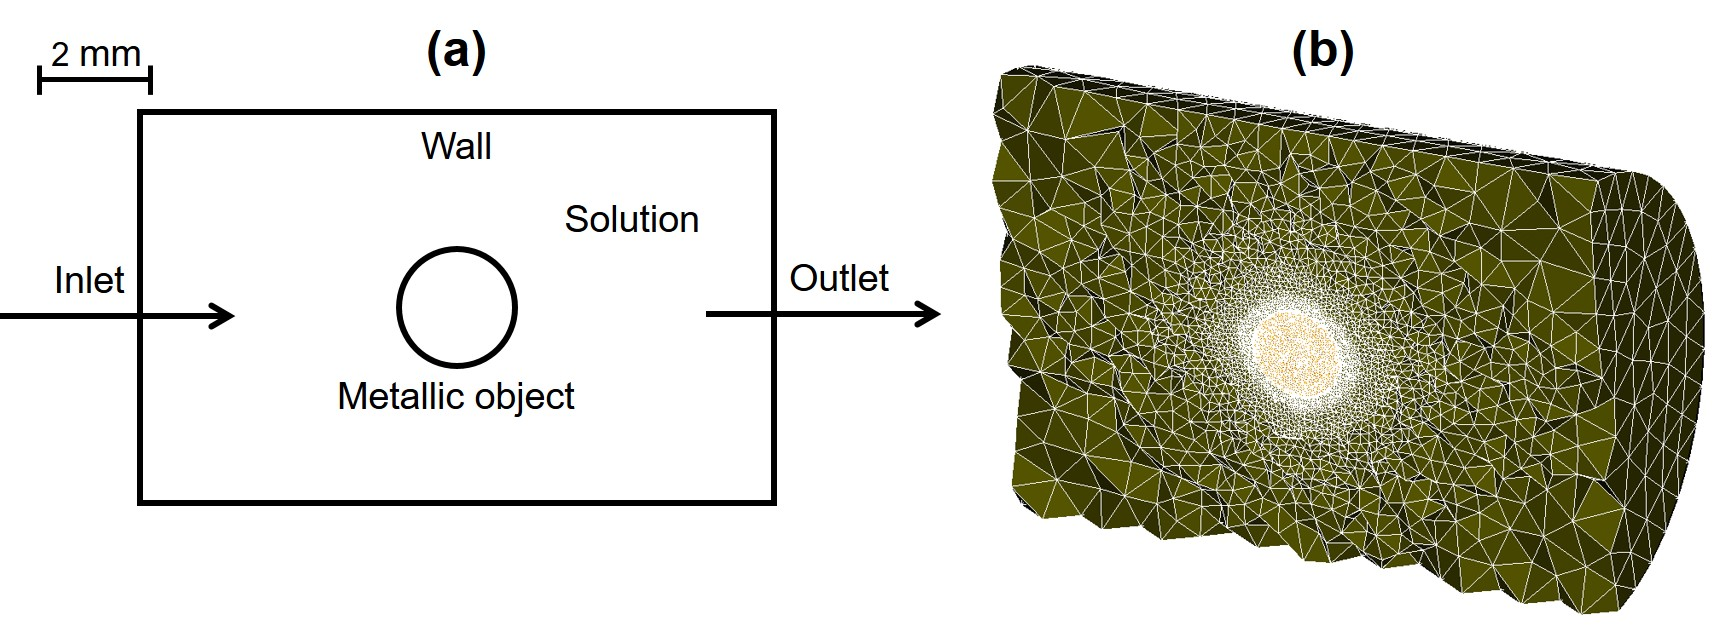
\includegraphics[width=\textwidth]{coupled_setup.jpg}
\caption[Model construction for checking the coupling of the fluid flow and biodegradation models]{Model construction for checking the coupling of the fluid flow and biodegradation models: a) schematic representation of the domain b) the generated computational mesh.} \label{fig:fluid_coupled_setup}
\end{figure}

Additionally, a simple 2D representation of the full chamber model (Fig. \ref{fig:fluid_setup}) was constructed to test the effect of the fluid flow on the degradation behavior of the metallic parts. In this model, a high inlet velocity and a high diffusion coefficient were used to have an exaggerated degradation, showing how the fluid flow would affect the change of morphology of the object. The degrading metallic part was selected to be a small rectangle on the bottom of the chamber. The domain setup is depicted schematically in Fig. \ref{fig:fluid_chamber_degrade_setup}. The computational mesh was generated using the SALOME platform and contained \num{24946} elements.

\begin{figure}[h]
\centering
\medskip
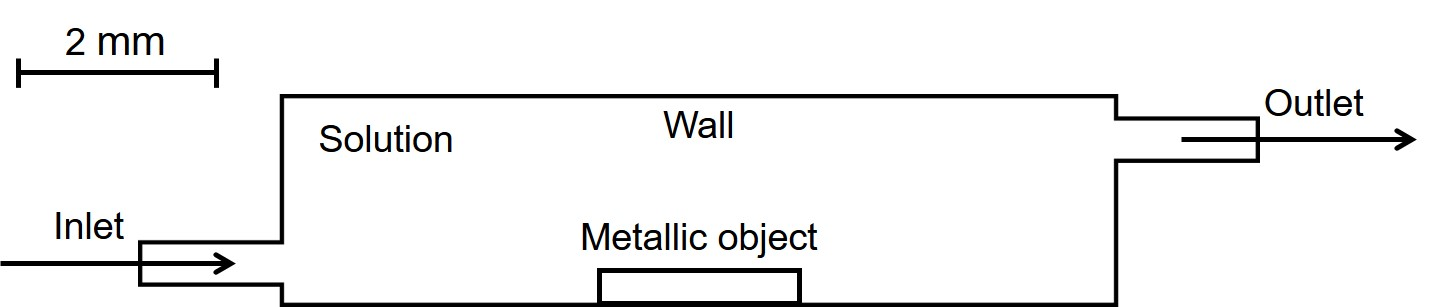
\includegraphics[width=0.8\textwidth]{chamber_degrade_setup.jpg}
\caption[Schematic view of the model for checking the effect of fluid flow on biodegradation behavior]{Schematic view of the model used for checking the effect of the fluid flow on biodegradation behavior.} \label{fig:fluid_chamber_degrade_setup}
\end{figure}

\section{Results}

To verify the robustness of the model predictions, the results of the \gls{CFD} code developed in FreeFEM were compared both quantitatively and qualitatively with an OpenFOAM model of an identical set-up. The qualitative comparison was made via the streamlines, showing how the flow develops by plotting the trajectory lines of the fluid velocity field inside the desired domain, which is the chamber in this case. Figs. \ref{fig:fluid_streamlines_side} and \ref{fig:fluid_streamlines_top} show such comparison between the developed model and OpenFOAM. Fig. \ref{fig:fluid_streamlines_side} shows the streamlines for both models from a side view, in which the flow enters the chamber from the left inlet pipe and leaves it from the top right outlet. The qualitative comparison shows a good agreement between the predictions of the models.

\begin{figure}[h]
\centering
\medskip
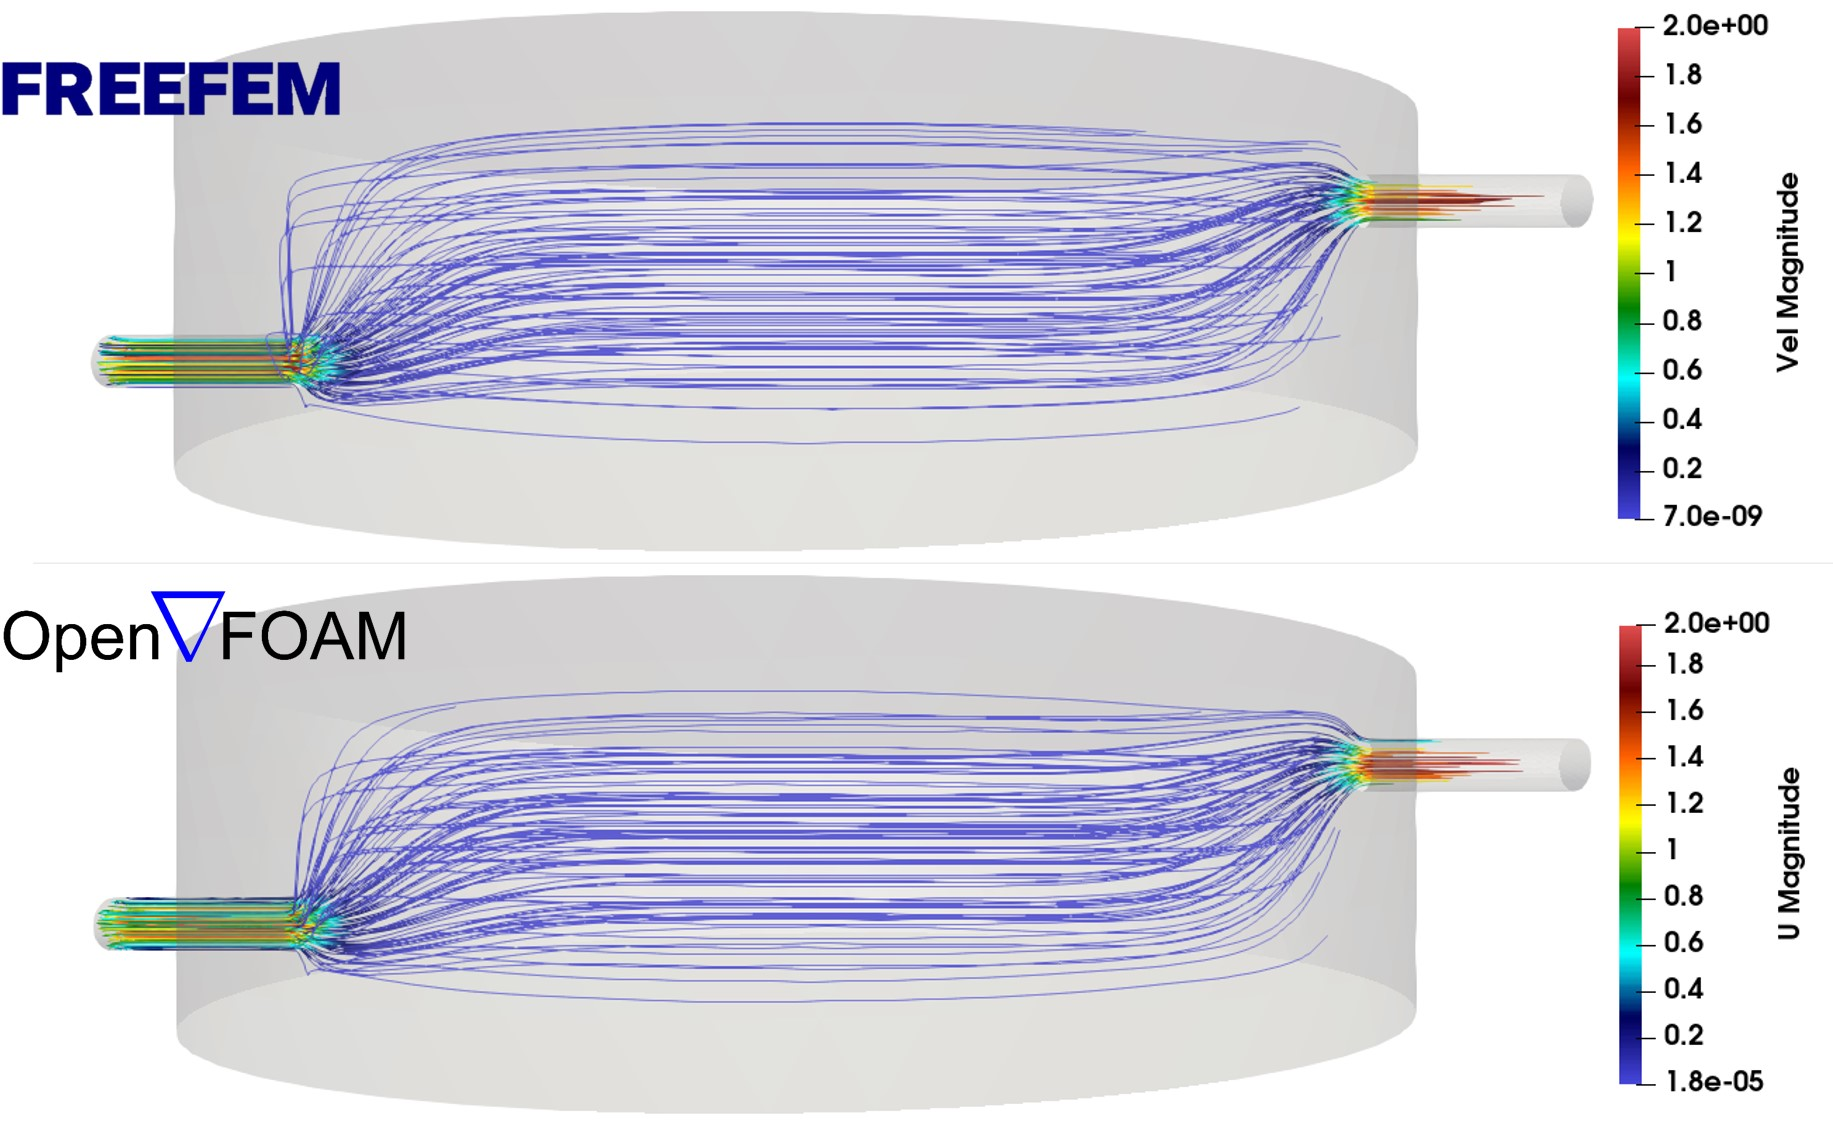
\includegraphics[width=\textwidth]{streamlines_side.jpg}
\caption[Comparing streamline results of developed CFD code and OpenFOAM - side view]{Comparing the results of the developed \gls{CFD} model (top) with OpenFOAM (bottom) via plotting the streamlines of the fluid velocity field, depicted from the side view. The colors on the trajectory lines show the magnitude of the velocity vector (in $\mathrm{mm}/\mathrm{s}$).} \label{fig:fluid_streamlines_side}
\end{figure}

Similarly, Fig. \ref{fig:fluid_streamlines_top} depicts a comparison but from the top view, showing good agreement between the predictions, although the OpenFOAM model (bottom) shows slightly better performance on the boundaries as can be appreciated from the existence of extra streamlines close to the cylinder boundary in the FreeFEM code results.

\begin{figure}[h]
\centering
\medskip
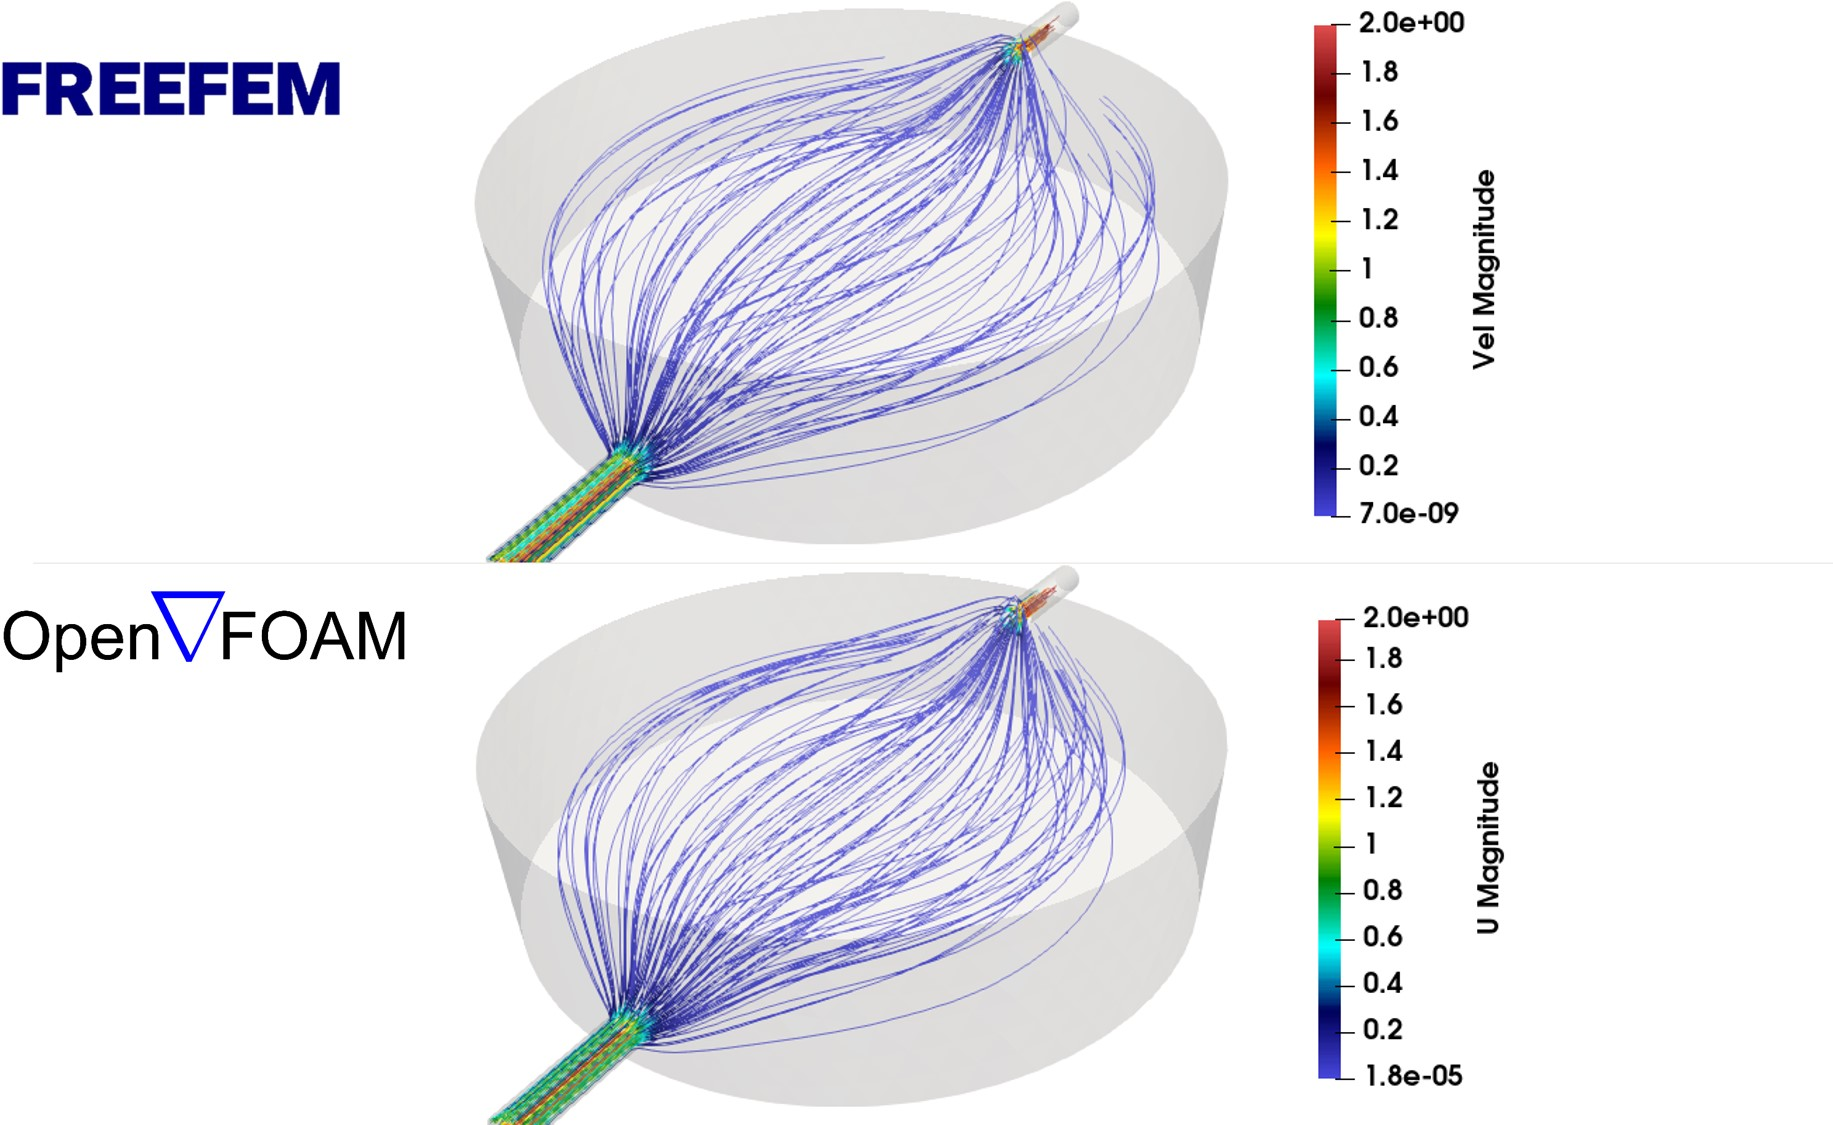
\includegraphics[width=\textwidth]{streamlines_top.jpg}
\caption[Comparing streamline results of developed CFD code and OpenFOAM - top view]{Streamlines of the fluid velocity field plotted from a top view to compare the output of the developed \gls{CFD} model (top) and OpenFOAM (bottom)  with colors showing the magnitude of the velocity vector at each point (in $\mathrm{mm}/\mathrm{s}$).} \label{fig:fluid_streamlines_top}
\end{figure}

Moreover, a quantitative comparison is possible by comparing the numerical values predicted by the models in various regions of the desired domain, including the regions close to the boundaries. Fig. \ref{fig:fluid_flow_chamber} shows the comparison of the fluid velocity field visualization between the developed \gls{CFD} code and OpenFOAM on a cross-section in the center of the chamber, showing that both models produce the same results quantitatively.

\begin{figure}[h]
\centering
\medskip
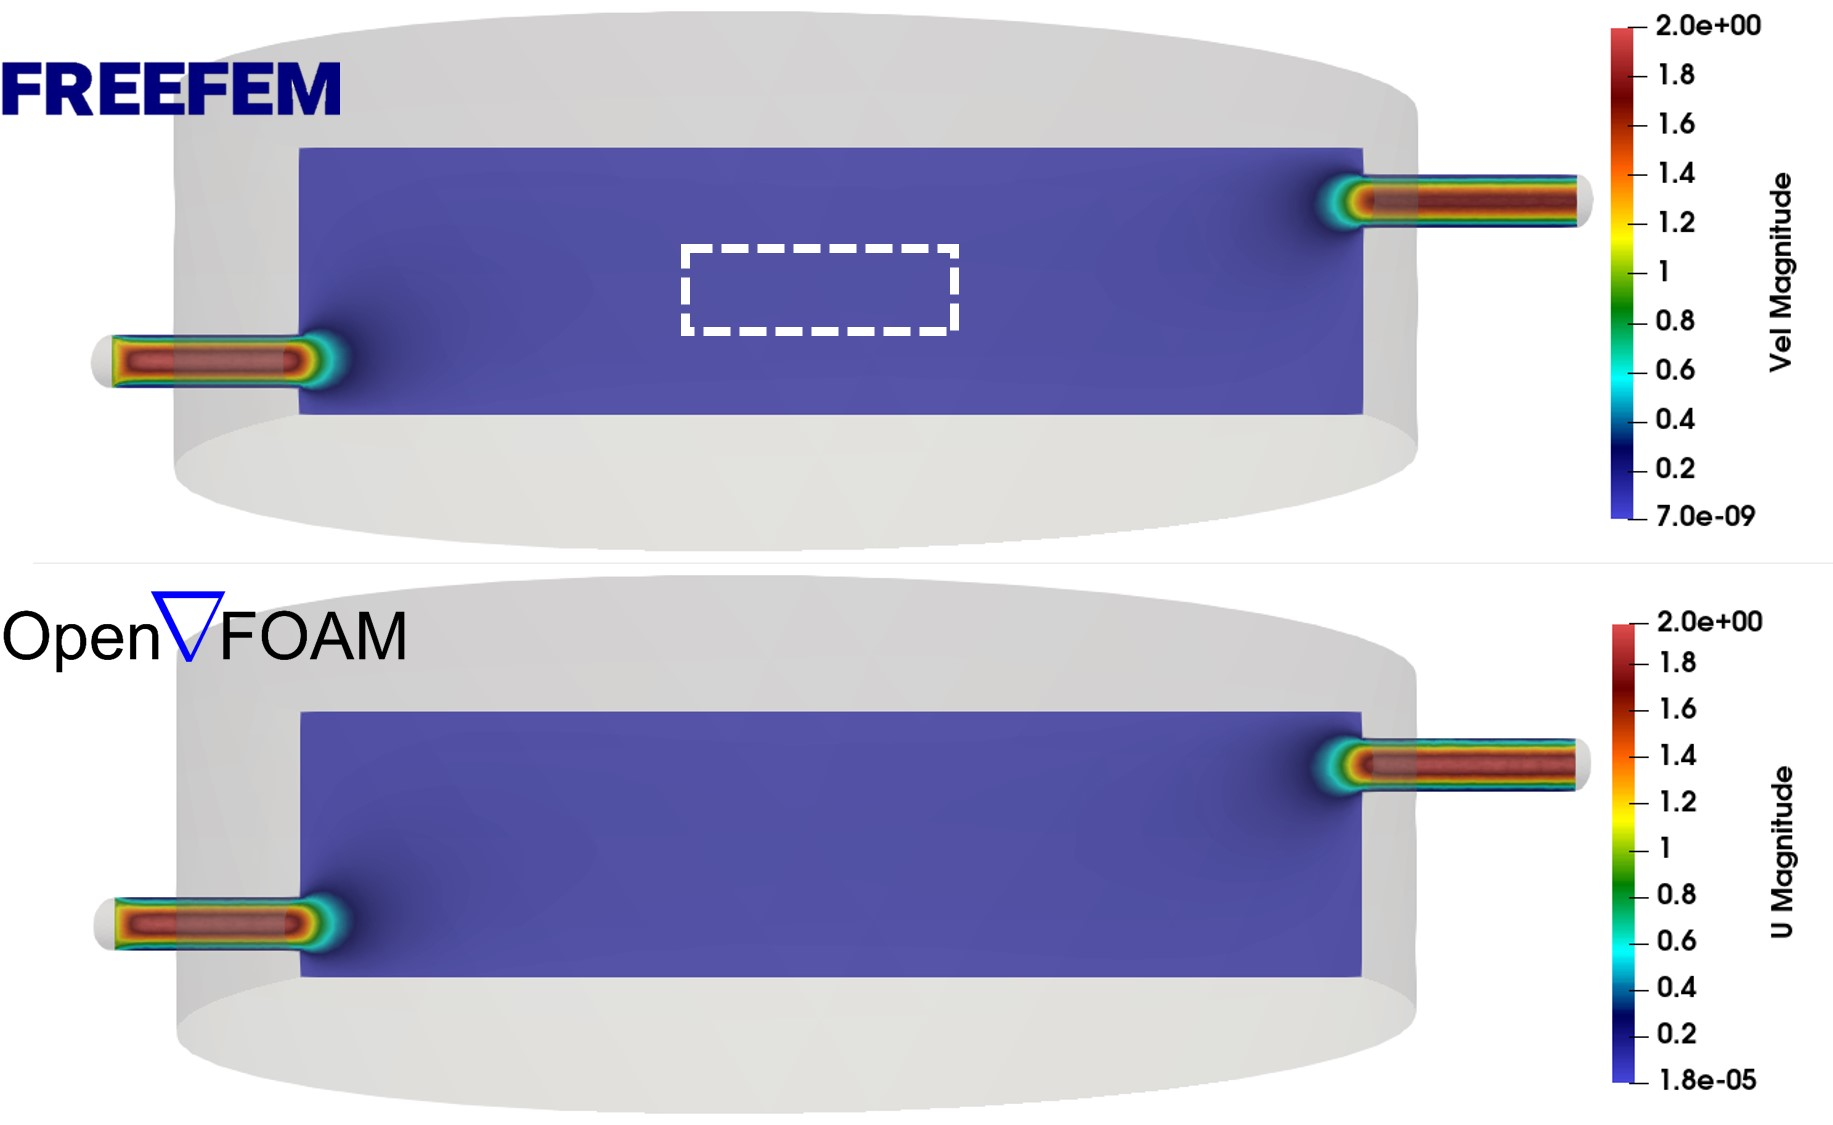
\includegraphics[width=\textwidth]{flow_chamber.jpg}
\caption[Comparing flow field results of developed CFD code and OpenFOAM]{comparison between the fluid velocity field predicted by the developed \gls{CFD} code (top) and OpenFOAM (bottom), depicted on a vertical cross-section in the center of the chamber. Fluid enters the chamber from the left and leaves it from the right. The colors show the magnitude of the velocity vector at each point (in $\mathrm{mm}/\mathrm{s}$). The white dashed-line box shows the zoomed-in area of Fig. \ref{fig:fluid_flow_chamber_zoom}.} \label{fig:fluid_flow_chamber}
\end{figure}

A closer look at the center of Fig. \ref{fig:fluid_flow_chamber} is depicted in Fig. \ref{fig:fluid_flow_chamber_zoom}, where the color bar range is adapted to contain only the visible values. This zoomed-in comparison confirms the good agreement between the \gls{CFD} model and OpenFOAM results. The employed mesh is relatively coarse in the center (regions far from the inlet and outlet), the effect of which can be seen as non-smooth velocity profiles in Fig. \ref{fig:fluid_flow_chamber_zoom}. Still, both models handle this coarse mesh effect similarly.

\begin{figure}[h]
\centering
\medskip
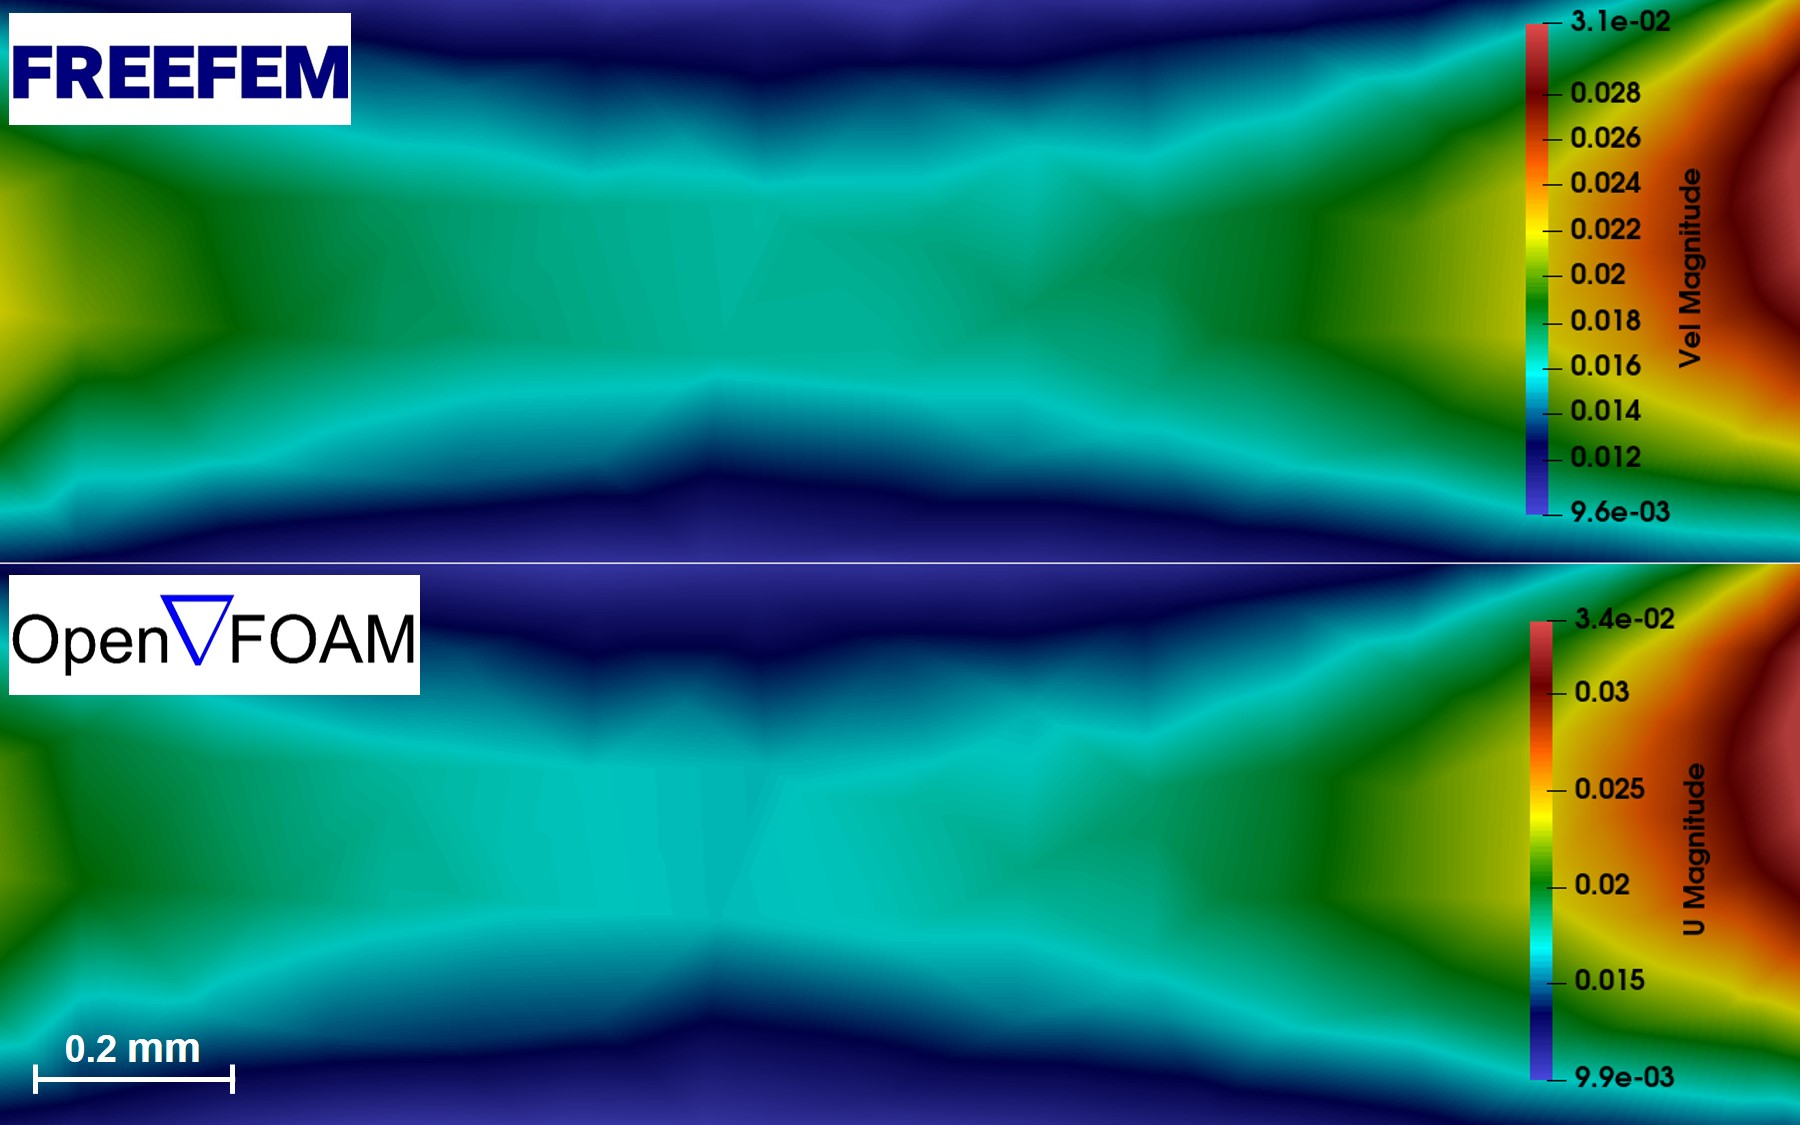
\includegraphics[width=\textwidth]{flow_chamber_zoom.jpg}
\caption[Comparing flow field results of developed CFD code and OpenFOAM - zoomed-in view]{A zoomed-in view of the area depicted as white dashed-line in Fig. \ref{fig:fluid_flow_chamber}, indicating the fluid velocity field for results predicted by the developed \gls{CFD} code (top) and OpenFOAM (bottom) with colors showing the magnitude of the velocity vector at each point (in $\mathrm{mm}/\mathrm{s}$).} \label{fig:fluid_flow_chamber_zoom}
\end{figure}

Fig. \ref{fig:fluid_flow_degrading} shows the result of a proof-of-concept simulation in which the biodegradation model \cite{Barzegari2021} (presented in Chapter \ref{ch:core}) is coupled with the fluid flow model. This was done by solving Eq. \ref{eq:fluid_ns_permeab} (or Eq. \ref{eq:fluid_stokes_permeab} for simpler cases) and adding a convection term to the equations of the biodegradation model to include the directional effect of fluid flow on the degrading object. The interplay between the fluid flow and the degradation can be seen in Fig. \ref{fig:fluid_flow_degrading} with the released ions being advected to the right (the direction of the fluid flow) and the degrading object being slightly more degraded on the left.

\begin{figure}[h]
\centering
\medskip
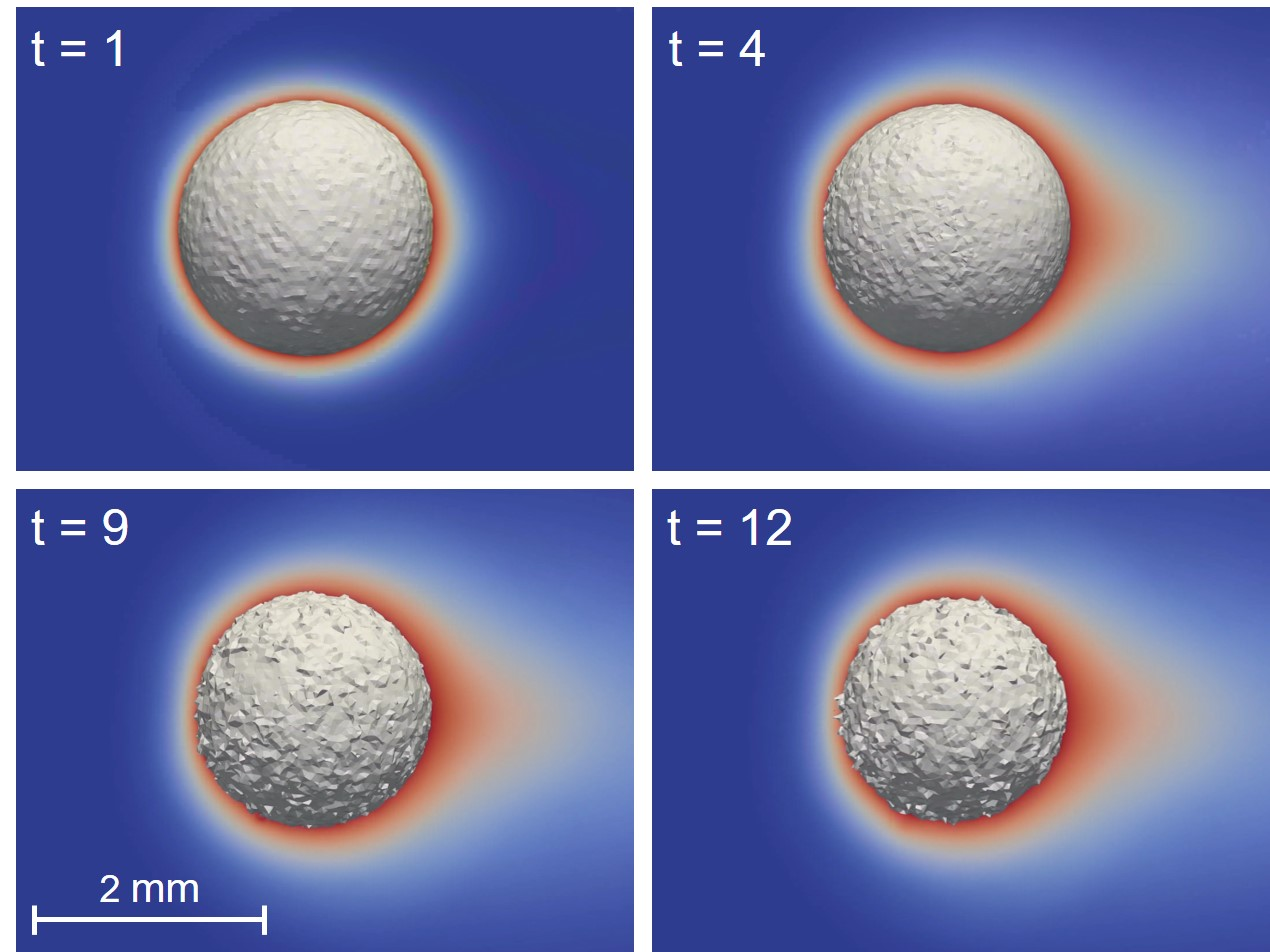
\includegraphics[width=\textwidth]{flow_degrading.jpg}
\caption[Biodegradation simulation results in the presence of fluid flow]{Biodegradation simulation results in the presence of fluid flow over time (in arbitrary units), showing the interplay between the fluid flow and biodegradation models. The flow gets detoured due to the presence of an obstacle, and the released ions get advected to the direction of fluid flow (left to right). The colors represent the concentration of Mg ions as they get released to the surrounding environment and subsequently get diffused/advected. The gray surface shows the zero iso-contour of the used level-set function to track the degrading object's interface, demonstrating the solid part's change of morphology.} \label{fig:fluid_flow_degrading}
\end{figure}

Fig. \ref{fig:fluid_flow_degrading_streamline} shows the effect of the degrading object on the fluid velocity field, depicted as streamlines passing over the solid part at the end of the performed simulation. The figure demonstrates the fluid flow response to the presence of the changing morphology of the obstacle, obtained from solving the Navier-Stokes equations containing the Darcy term (Eq. \ref{eq:fluid_ns_permeab}).


\begin{figure}[h]
\centering
\medskip
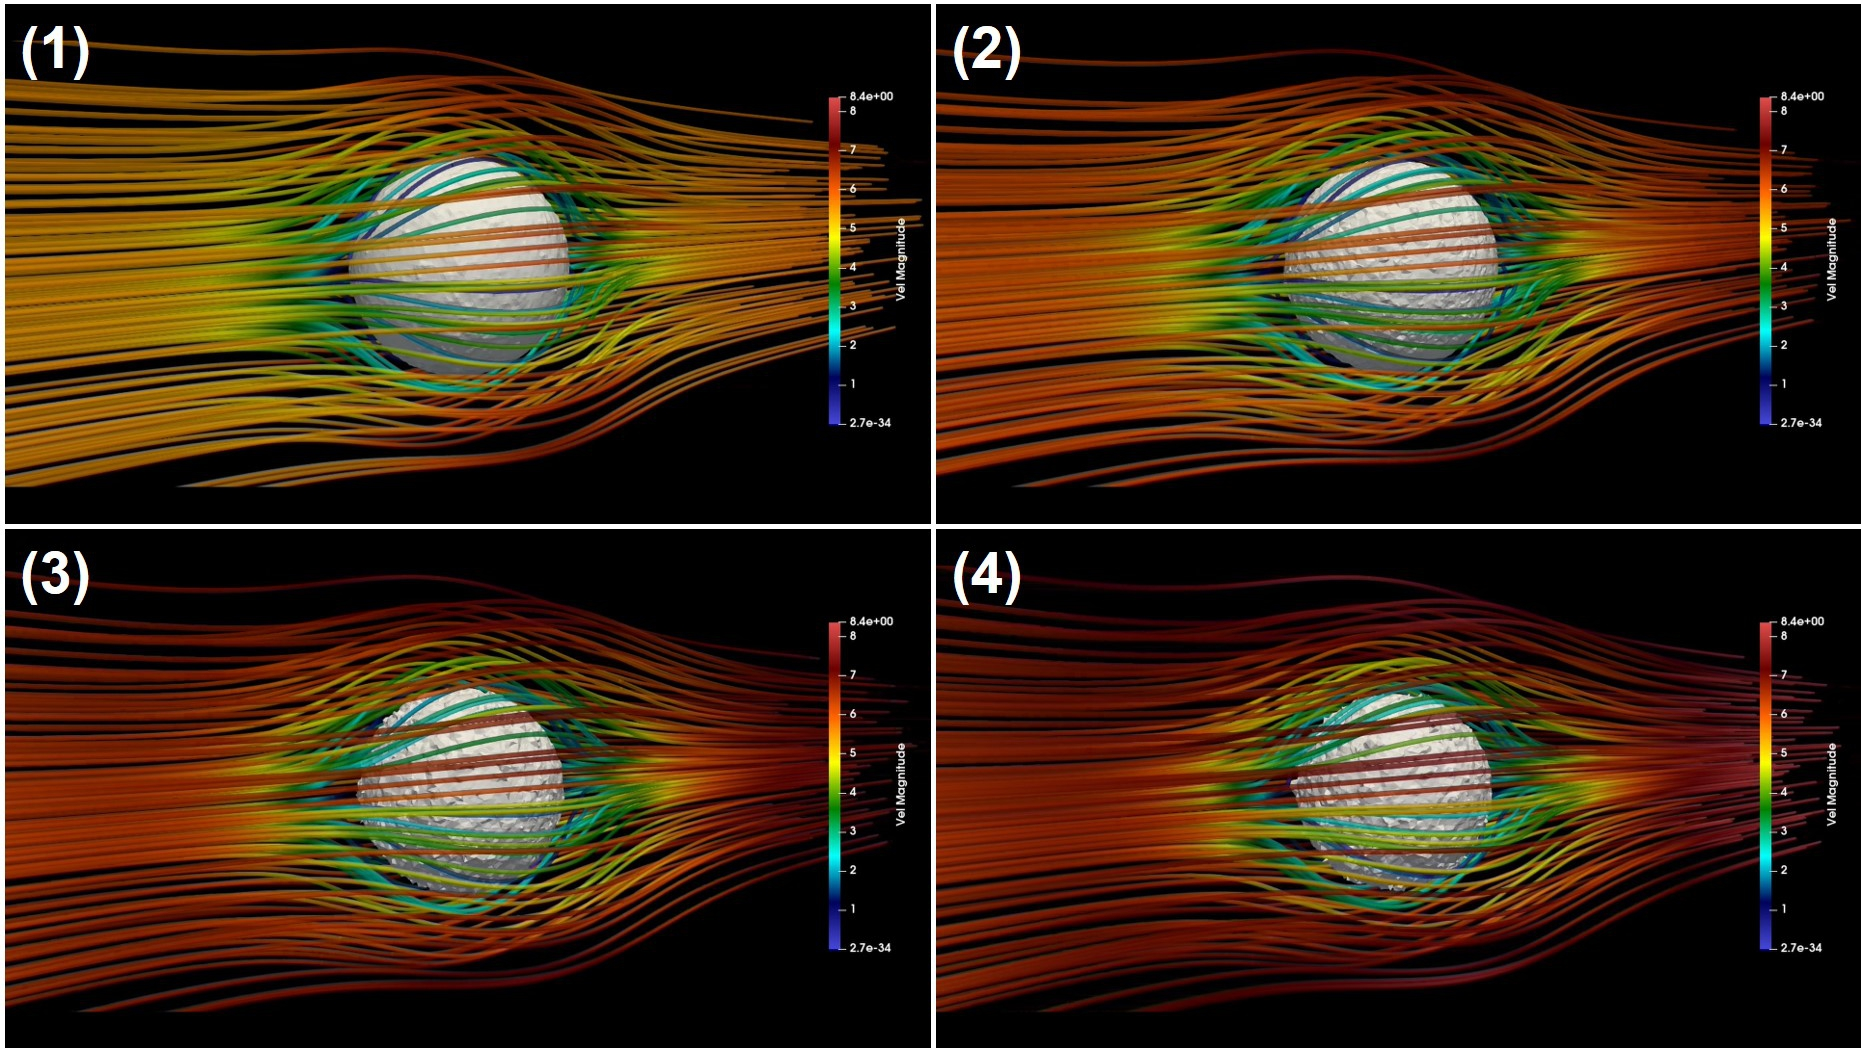
\includegraphics[width=\textwidth]{flow_degrading_streamline.jpg}
\caption[Fluid flow streamlines in the presence of a degrading object]{Visualization of the fluid velocity field depicted by streamlines passing over a degrading object. Colors show the magnitude of the velocity field (in $\mathrm{mm}/\mathrm{s}$) projected on the streamlines.} \label{fig:fluid_flow_degrading_streamline}
\end{figure}


Fig. \ref{fig:fluid_degradation_chamber} shows the results of the second test case for the coupled biodegradation model, in which the release of metallic ions is depicted over time along with the change of the morphology of the degrading object. The released metallic ions get convected in the direction of the flow field inside the chamber, which was obtained by solving the Navier-Stokes equations.


\begin{figure}[h]
\centering
\medskip
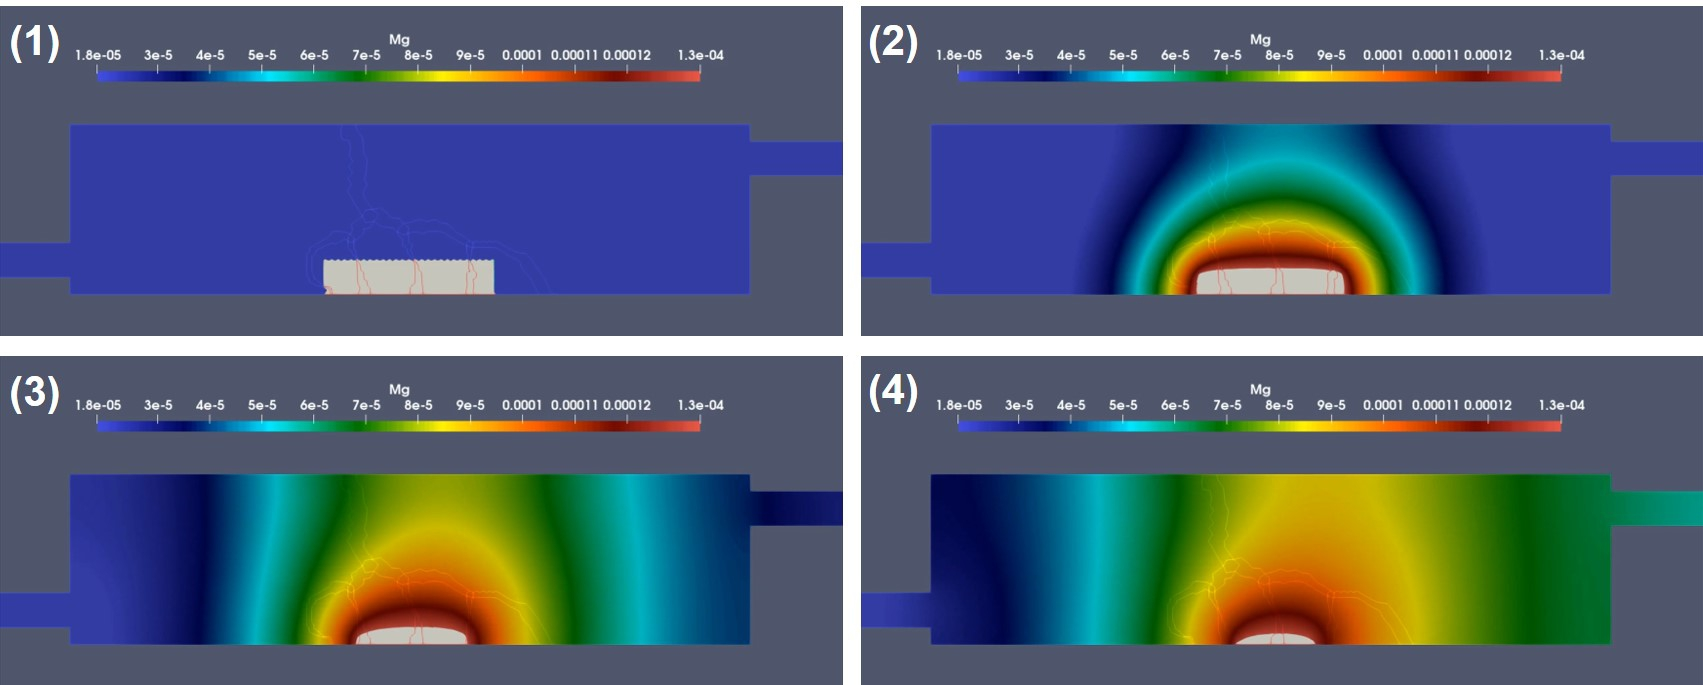
\includegraphics[width=\textwidth]{degradation_chamber.jpg}
\caption[Visualization of the biodegradation inside the chamber in the presence of fluid flow]{Visualization of the results of the biodegradation of an object inside the chamber in hydrodynamics conditions. Colors show the concentration of released metal ions getting convected in the direction of fluid flow. The light gray part shows the degrading object.} \label{fig:fluid_degradation_chamber}
\end{figure}


\section{Discussion}


In this study, a parallel fluid flow model was developed to be coupled with the computational biodegradation model enabling the consideration of the effect of the hydrodynamics conditions in corrosion tests. The most important form of hydrodynamics in tissue engineering is the perfusion phenomenon in bioreactors, which makes the development of such coupled degradation-\gls{CFD} model even more crucial considering the final application of the biodegradation model. Similar to perfusion bioreactors, the hydrodynamics set-up in biodegradation tests helps removing corrosion products and providing mechanical forces if applicable.


In order to verify the developed \gls{CFD} model, a test case was prepared to simulate a similar chamber flow model in both the in-house FreeFEM code and the OpenFOAM code, a well-established open-source \gls{CFD} solver. Qualitative (Figs. \ref{fig:fluid_streamlines_side} and \ref{fig:fluid_streamlines_top}) and quantitative (Figs. \ref{fig:fluid_flow_chamber} and \ref{fig:fluid_flow_chamber_zoom}) comparison of results show identical predictions for the flow field in both models, demonstrating that the derivation of the weak forms of Navier-Stokes equations as well as their numerical implementation in FreeFEM were performed correctly. This comparison indicates that the developed code can be used instead of a well-known and sophisticated \gls{CFD} solver for the desired flow regime, which is laminar flow with low Reynolds numbers.

\newglossaryentry{IO}{name={IO},description={input output}}

The reason for developing an in-house \gls{CFD} code instead of using a well-established \gls{CFD} solver lies in the lack of availability of proper coupling software. Although various efficient solver coupling codes exist and are widely used in similar scenarios (such as the preCISE coupling library \cite{preCICEv2}), at the time of this writing and to the best of the authors' knowledge, there is no compatible coupling software for FreeFEM, the language in which the computational model of the biodegradation process was implemented. In case of existence, the computational biodegradation model could have been linked with OpenFOAM, SU2, or Code\_Saturne in an efficient in-memory way. But, with such an approach not available, the only feasible approach would be coupling the models using disk \gls{IO} (input-output), meaning that in each time step, the computational model should write the domain data on disk (we should notice that the domain evolves since it is a moving interface problem), and the \gls{CFD} code reads the data, computes the flow field, and writes it back to the disk so that the biodegradation would read it back. Despite the possibility of employing this approach, the computationally intensive aspects of the models, which is the result of a 3D mesh refined on the corrosion interface leading to normally 2M-4M elements, makes the workflow dramatically inefficient. Working in \gls{HPC} environments and dealing with a partitioned mesh can make the situation even more complex. This reasoning made it inevitable to develop an in-house \gls{CFD} code so that it can be seamlessly and efficiently coupled with other models.

In order to couple the flow model with the computational biodegradation model, both models should be modified to include the effect of the other one. For the biodegradation model, the effect of fluid flow was considered as an extra convection term in the set of derived reaction-diffusion equations, which can be implemented using the method of characteristics in FreeFEM. On the other side, the inclusion of the effect of a degrading object can be more tricky in the \gls{CFD} model. This was done by adding a Darcy term to the Navier-Stokes and Stokes equation, which considers a high permeability for the regions inside the degrading object, preventing fluid from penetrating into those parts. After the degrading part interface shrinks, the Darcy term gets updated automatically since it is formulated based on the level-set function used in the biodegradation model to describe the moving corrosion interface. Figs. \ref{fig:fluid_flow_degrading} and \ref{fig:fluid_flow_degrading_streamline} demonstrate the effect of the presence of the degrading part on the pattern of flow, while Fig.
\ref{fig:fluid_degradation_chamber} shows the effect of fluid flow on the biodegradation, which is the ions being convected in the direction of the fluid velocity field, leading to a minor directional degradation in which the side facing the flow direction degrades slightly faster.

The performed verification study on the developed CFD code is not enough to call it a fully validated fluid flow model. However, by considering the desired flow regime in biodegradation tests, the verification shows that the coupled model is capable of predicting acceptable and correct results. Nonetheless, dedicated validation tests can be further done to fully validate the developed model as a general CFD code which can be used standalone for simulating laminar flows with low Reynolds numbers.













%%%%%%%%%%%%%%%%%%%%%%%%%%%%%%%%%%%%%%%%%%%%%%%%%%
% Keep the following \cleardoublepage at the end of this file,
% otherwise \includeonly includes empty pages.
\cleardoublepage
